\documentclass[../main]{subfiles}
\graphicspath{{\subfix{../Images/}}}

\begin{document}

\section*{Załącznik nr 1: System wbudowany}\addcontentsline{toc}{section}{Załącznik nr 1: System wbudowany}\label{sec:zalacznik-1}

Skoro nie ma jednoznacznej definicji pojęcia "system wbudowany", należy określić definicję, która jest wykorzystywana w tej pracę.

System wbudowany jest systemem, to znaczy ma cechy systemu: jest złożony z więcej niż jednego elementu, jest funkcjonalnie niezależny od środowiska i posiada możliwość reagowania (tzn. odbierania, przetwarzania i udzielenia odpowiedzi) na bodźce zewnętrzne. "Wbudowany" oznacza, że system jest częścią innego systemu fizycznie i/lub funkcjonalnie.

Natomiast przełożyć tę definicję na dziedzinę elektroniki i informatyki można w następujący sposób: system wbudowany — jest to system komputerowy składający się z jednostki obliczeniowej i modułów wejścia/wyjścia (tzn. może reagować na bodźce zewnętrzne), mający wszystkie narzędzia, w tym oprogramowanie, do pełnienia pewnej, zdefiniowanej funkcji (więc może być wyodrębniony) i będący częścią większego systemu.
% TODO: Nie cytuję tu rzadnej książki ani normy, bazuję sie na swojej wiedzę, ale agólnie ta definicja jest podobna od książki do książki.

\section*{Załącznik nr 2: Wirtualizacja}\addcontentsline{toc}{section}{Załącznik nr 2: Wirtualzacja}\label{sec:zalacznik-2}

Wirtualizacja jest technologią wprowadzającą separację środowisk z oprogramowaniem poprzez tworzenie tzw. \gls{vm} zarządzanych przez \gls{vmm} (\cref{fig:virt}). Rodzaje separacji używane w wirtualizacji to: separacja pamięciowa (poprzez translację pamięci), separacja sygnałowa (przekierowywanie przerwań) i separacja stanów (przełączanie kontekstu).

Celem separacji pamięciowej jest przypisanie do każdej \gls{vm} przedziału adresów pamięci (kodu programu i urządzeń peryferyjnych, ponieważ rejestry tych urządzeń są zmapowane do pamięci; ang. memory-mapped peripherals) oraz wychwytywanie wszystkich prób manipulacji pamięcią, która nie jest przypisana do tej \gls{vm}. W architekturach \gls{arm} tym zajmuje się \gls{mmu}, który, począwszy od \gls{arm}v8, posiada dwa poziomy translacji: z poziomu aplikacji, tzw. \gls{va}, do poziomu systemu operacyjnego, tzw. \gls{ipa}, i do poziomu hiperwizora, tzw. \gls{pa}.

Celem separacji sygnałowej jest podział i przekierowywanie przerwań sprzętowych pomiędzy \gls{vm}. Każda \gls{vm} ma przepisany podzbiór urządzeń peryferyjnych za pomocą separacji pamięci. Te urządzenia mogą generować przerwania, za przekierowywanie których jest odpowiedzialny hiperwizor i kontroler przerwań, w przypadku \gls{arm}'u to jest \gls{gic}.

Celem separacji stanów jest sprzętowy podział wykonywanych programów i przypisanie do nich odpowiednich poziomów uprawnień. Dokładniej to jest opisane w \hyperref[sec:zalacznik-3]{załączniku nr 3}.

Przy czym, typowo hiperwizor jest zaprojektowany w taki sposób, że przy użyciu wszystkich tych rodzajów separacji aplikacja (lub system operacyjny), uruchomiana na tym hiperwizorze wcale nie musi wiedzieć, że jest uruchomiana nie wprost na rzeczywistym sprzęcie. Taki rodzaj wirtualizacji nazywany jest wirtualizacją natywną (ang. native virtualization, także ang. full virtualization, lub ang. hardware-accelerated virtualization).

W przypadku, gdy sprzęt nie posiada dedykowanych narzędzi do zapewnienia jednego z rodzajów separacji, można skorzystać z tzw. parawirtualizacji (ang. paravirtualization). W takim przypadku aplikacja, która jest uruchamiana na hiperwizorze, jest modyfikowana w sposób taki, aby wiedziała, że nie działa na realnym sprzęcie, a na wirtualnym, i była świadoma obecności hiperwizora. Przykładem może być separacja pamięciowa. Typowo próba otrzymania dostępu do zabronionej sekcji pamięci RAM jest wykrywana przez \gls{mmu}. W przypadku nieobecności tego modułu aplikacja jest modyfikowana, co oznacza, że wszystkie instrukcje odczytujące dane z pamięci są podmieniane na zestaw instrukcji, który powoduje komunikat do hiperwizora w celu sprawdzenia dostępów. 

\section*{Załącznik nr 3: Przełączanie stanu i kontekstu, definicja procesu}\addcontentsline{toc}{section}{Załącznik nr 3: Przęłączanie stanu i kontekstu, definicja procesu}\label{sec:zalacznik-3}

Na początku należy oddzielić pojęcie programu od pojęcia procesu. Program, w przypadku oprogramowania, to jest lista instrukcji do wykonania przechowywana w dowolnym miejscu. Program nie posiada, żadnego stanu, po prostu istnieje. Natomiast procesem jest program z przydzielonym stanem. Każdy stan procesu może zawierać dodatkowe dane, np. priorytet, zasoby, połączenia z innymi procesami i tak dalej. Na \cref{fig:process-states} jest pokazany najbardziej popularne stany procesu oraz przejścia pomiędzy nimi.

Stan wykonywanego oprogramowania określany jest przez następujące elementy:

\begin{itemize}
    \item Zawartości rejestrów ogólnego przeznaczenia: zawierają wyniki wykonywania ostatnich instrukcji;
    \item Rejestry wskazujące na adres następnej komendy (PC w architekturach \gls{arm}'owych), adres powrotu (LR w architekturach \gls{arm}'owych) i adres aktualnie używanego stosu (MSP lub PSP w architekturach \gls{arm}): określają "kierunek" (tzn. co będzie wykonane następne, gdzie wrócić po wykonaniu i tak dalej) wykonywanych instrukcji programu;
    \item Zawartość aktualnie używanego stosu: podobnie ja i w poprzednim punkcie, określa "kierunek" wykonywania instrukcji programu, przechowuje historie wykonywanych instrukcji programu (np. przy przerwaniu, do niego są zapisywane pewne rejestry, które po zakończeniu przerwania są odczytywane z powrotem, pozwalając na wznowienie wykonywanego programu);
    \item Rejestry systemowe (np. PSR i rejestry masek przerwań w architekturach \gls{arm}'owych): określają między innymi tryb jednostki obliczeniowej, w którym program jest wykonywany, co z olei określa poziom dostępu do zasobów sprzętowych. 
\end{itemize}

\begin{figure}[ht]
    \centering
    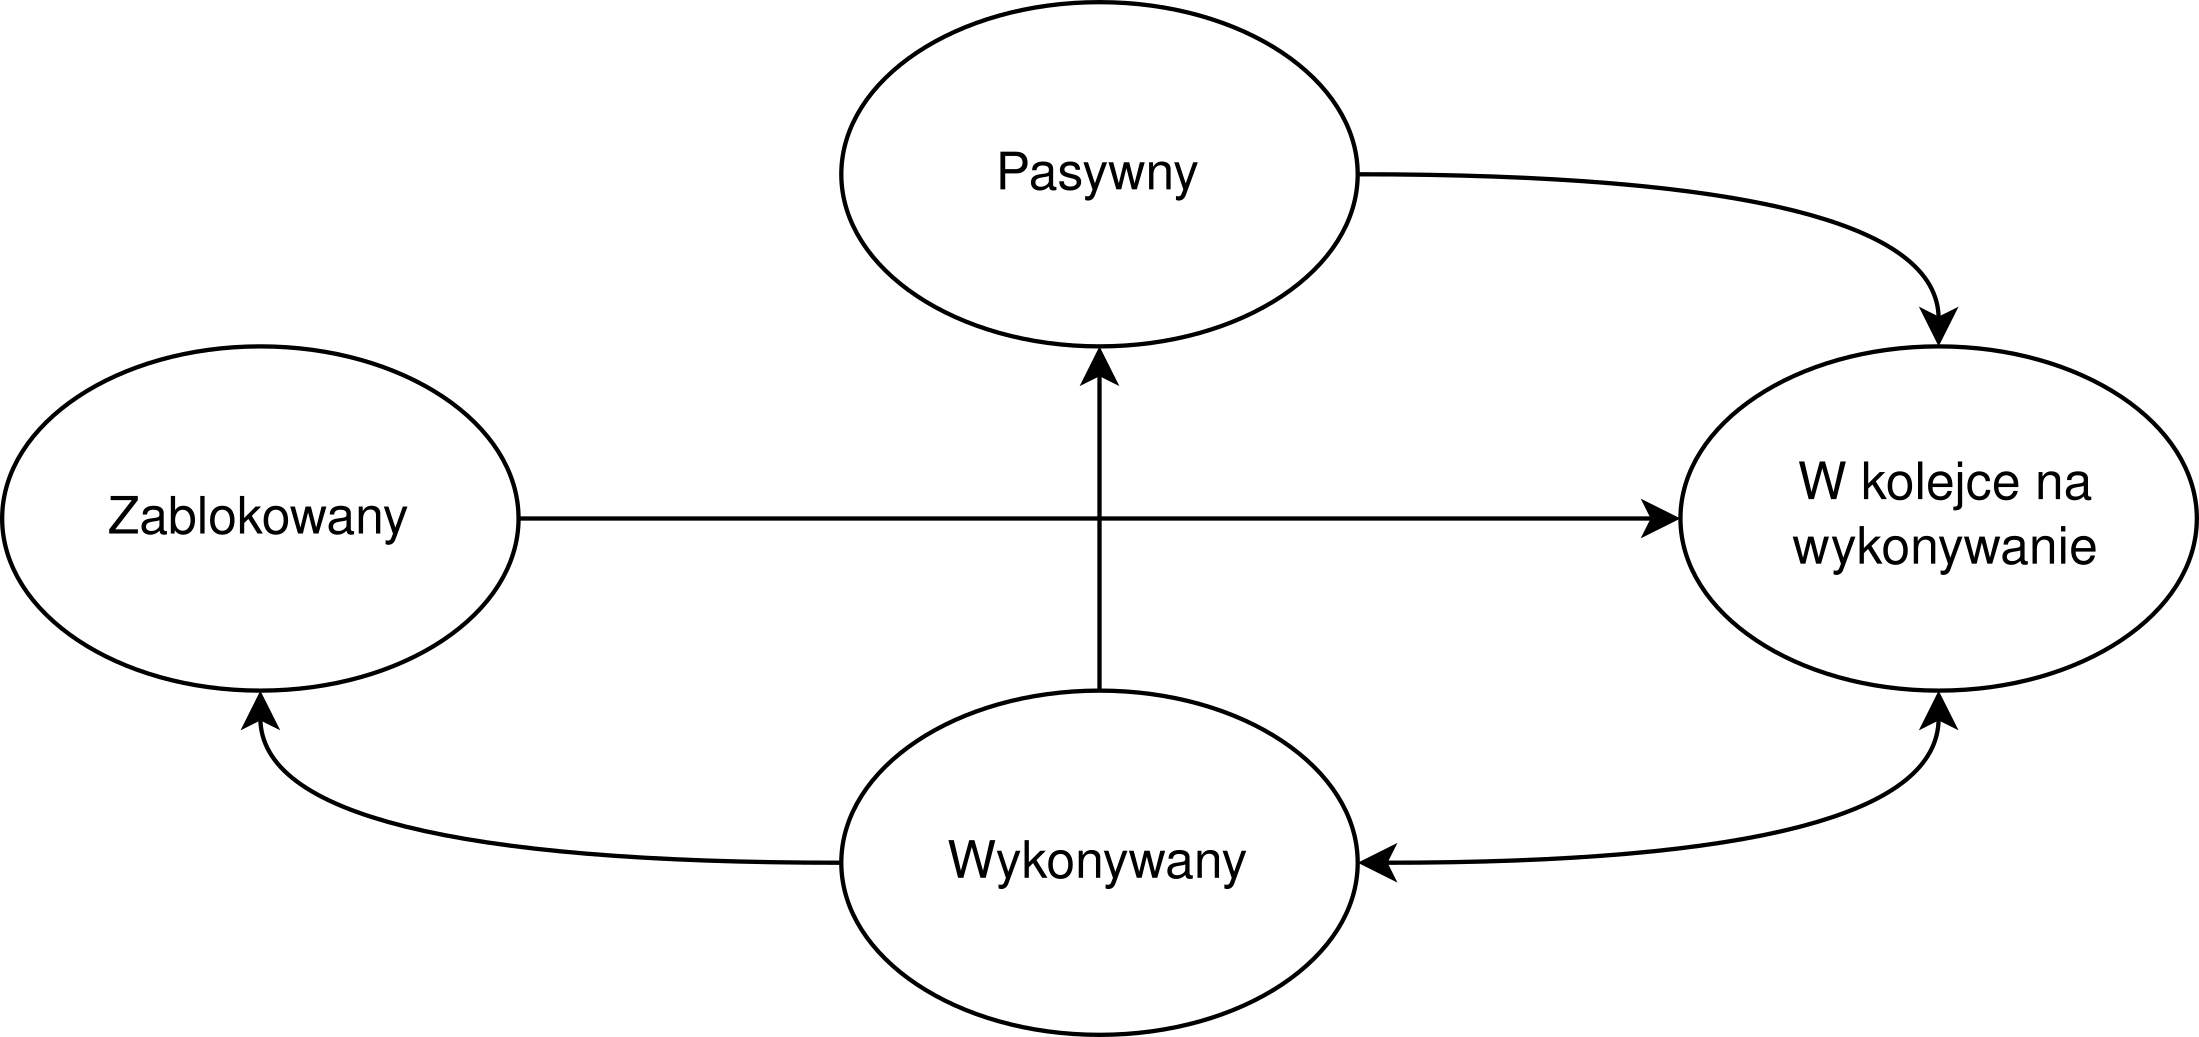
\includegraphics[width=0.85\textwidth]{Images/process-states.png}
    \caption{Ogólny graf stanów procesu}
    \label{fig:process-states}
\end{figure}

Z powyższego wynika, że stan wykonywanego oprogramowania to zbiór pewnych wartości przechowywanych w rejestrach jednostki obliczeniowej, co oznacza, że przełączenie stanów odbywa się sprzętowo, przez jednostkę obliczeniową, ponieważ oprogramowanie nie ma dostępu do zapisu ani odczytu wszystkich rejestrów jednostki obliczeniowej.

\begin{figure}[ht]
    \centering
    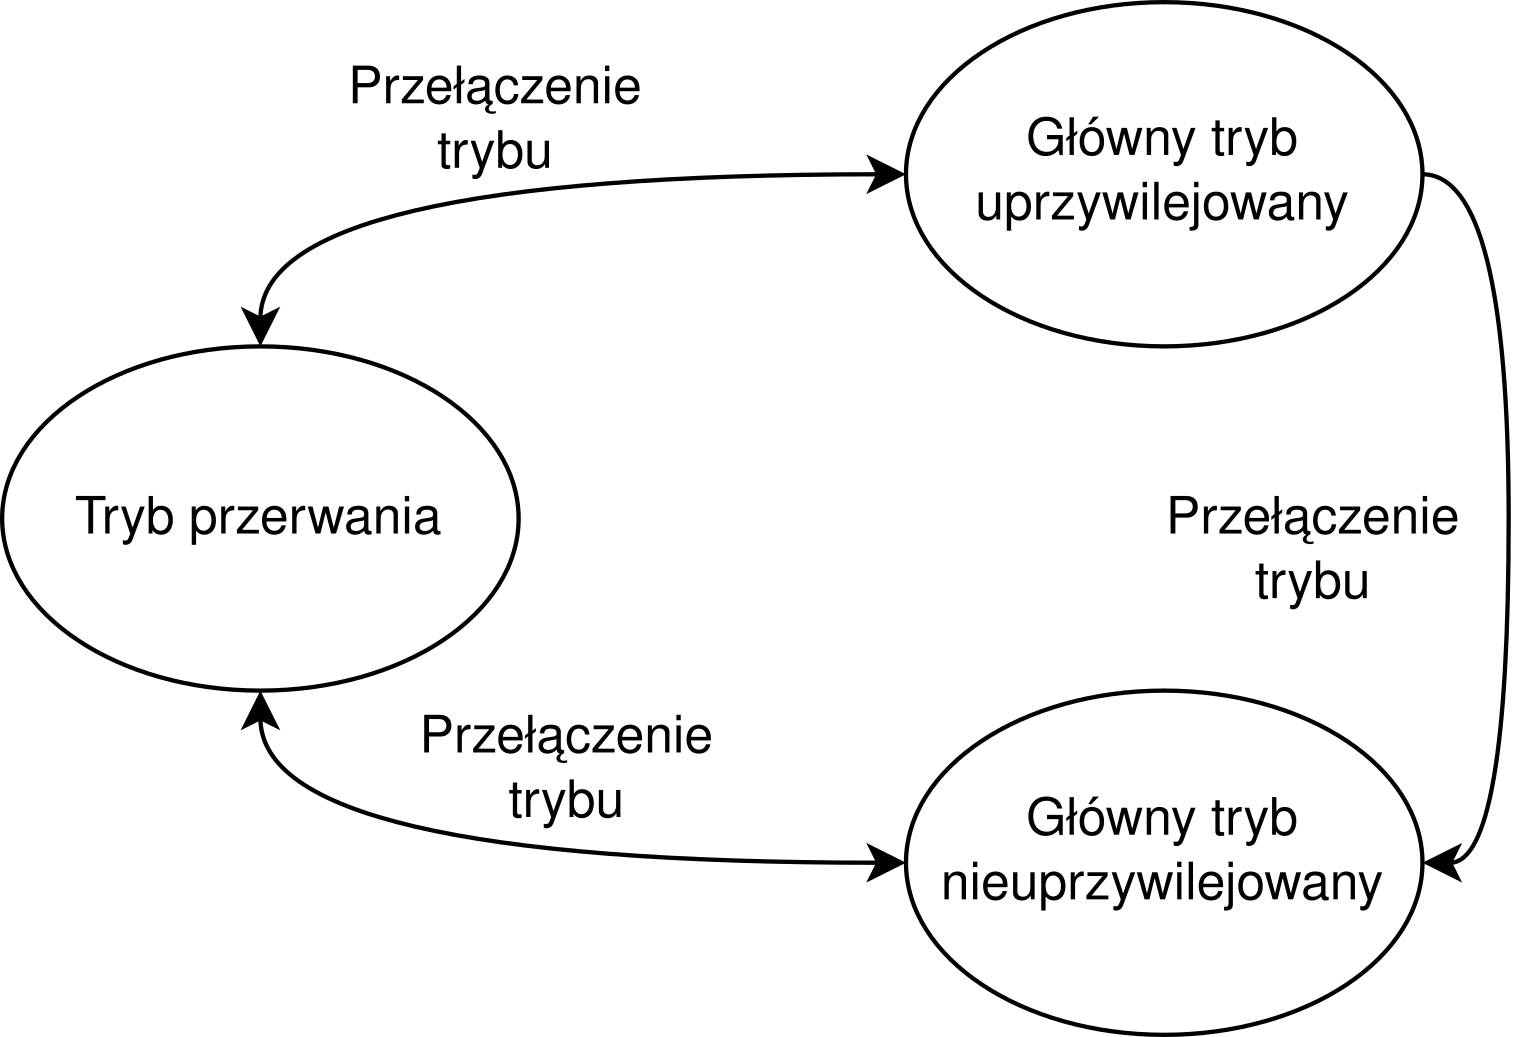
\includegraphics[width=0.7\textwidth]{Images/armv8m-modes.png}
    \caption{Tryby procesora zbudowanego na podstawie architektury ARMv8M
    \cite{armv8mintro}}
    \label{fig:armv8-m-modes}
\end{figure}

Z kolei przełączenie stanów to proces, w którym stan aktualnie wykonywanego oprogramowania jest zapisywany w stos przynależącego do tego oprogramowania i podmieniany na stan przynależący do innego oprogramowania, który jest odczytywany ze stosu uruchamianego oprogramowania. Występuje to podczas zmiany trybu jednostki obliczeniowej, ponieważ każdy tryb jednostki obliczeniowej ma własny stos.

Na \cref{fig:armv8-m-modes} pokazane są tryby jednostki obliczeniowej zbudowanej na podstawie architektury \gls{arm}v8M. Taka jednostka posiada trzy tryby z dwoma poziomami  dostępu: tryb główny uprzywilejowany, główny nieuprzywilejowany i tryb przerwania. Każdy z tych trybów ma swój stos, w którym jest przechowywany stan aktualnie wykonywanego oprogramowania. Adres każdego ze stosów jest przechowywany w rejestrach MSP i PSP \cite{armv8mintro}.

Natomiast kontekst programu to pojęcie zdefiniowane przez poszczególną implementację oprogramowania systemowego (system operacyjny bądź hiperwizor) i zawiera w sobie opisany wyżej stan programu oraz dodatkowe dane, interpretowane przez oprogramowanie systemowe (np. czas jednostki obliczeniowej użyty przez ten program, lub priorytet), zwane także metadanymi.

Stąd przełączenie kontekstu oznacza, że to nie jednostka obliczeniowa jest odpowiedzialna za wybór i uruchomienie programu, lecz oprogramowanie systemowe.

Na \cref{fig:armv8-m-context-switch} pokazano przykładowy przebieg takiego przełączenia dla architektury \gls{arm}v8M. Przełączenie kontekstu następuje podczas wykonywania kodu systemu operacyjnego, tzn. gdy jednostka obliczeniowa znajduje się w trybie głównym uprzywilejowanym (\cref{fig:armv8-m-modes}), co oznacza, że przed przełączeniem kontekstu następuje przełączenie stanów, podczas którego jednostka obliczeniowa przełącza się z wykonywania kodu aktualnego programu na wykonywanie kodu systemu operacyjnego (czyli przechodzi z trybu głównego nieuprzywilejowanego do trybu głównego uprzywilejowanego, \cref{fig:armv8-m-modes}). Natomiast po przełączeniu kontekstu następuje przełączenie stanów, podczas którego jednostka obliczeniowa przełącza się z wykonywania kodu systemu operacyjnego na wykonywanie kodu programu zaproponowanego przez system operacyjny podczas przełączenia kontekstu programu (tzn. przechodzi z trybu głównego uprzywilejowanego do trybu głównego nieuprzywilejowanego).

\section*{Załącznik nr 4: Zasób jednostki obliczeniowej}\addcontentsline{toc}{section}{Załącznik nr 4: Zasób jednostki obliczeniowej}\label{sec:zalacznik-4}

Jednostka obliczeniowa jest systemem, który przyjmuje instrukcje, wykonuje je i podaje wynik. Podstawową wielkością w tym przypadku będzie czas wykonania jednej instrukcji (w przypadku architektury \gls{risc} większość instrukcji są wykonywane w przedziale jednego okresu zegara zasilającego jednostkę obliczeniową).

Każdy program wykonywany przez jednostkę obliczeniową jest listą instrukcji, i każdemu programu zależy, aby ta lista instrukcji była wykonana jak najszybciej, czyli idealnie, jakby jedna jednostka obliczeniowa wykonywała tylko jeden program. Z tego wynika, że programy walczą o czas, na który im pozwolono używać jednostki obliczeniową do wykonania swoich instrukcji. Finalnie zasobem jednostki obliczeniowej jest czas.

Czas ten można podzielić pomiędzy programy w różny sposób, za to odpowiada nadzorca w oprogramowaniu systemowym.

\begin{figure}[ht]
    \centering
    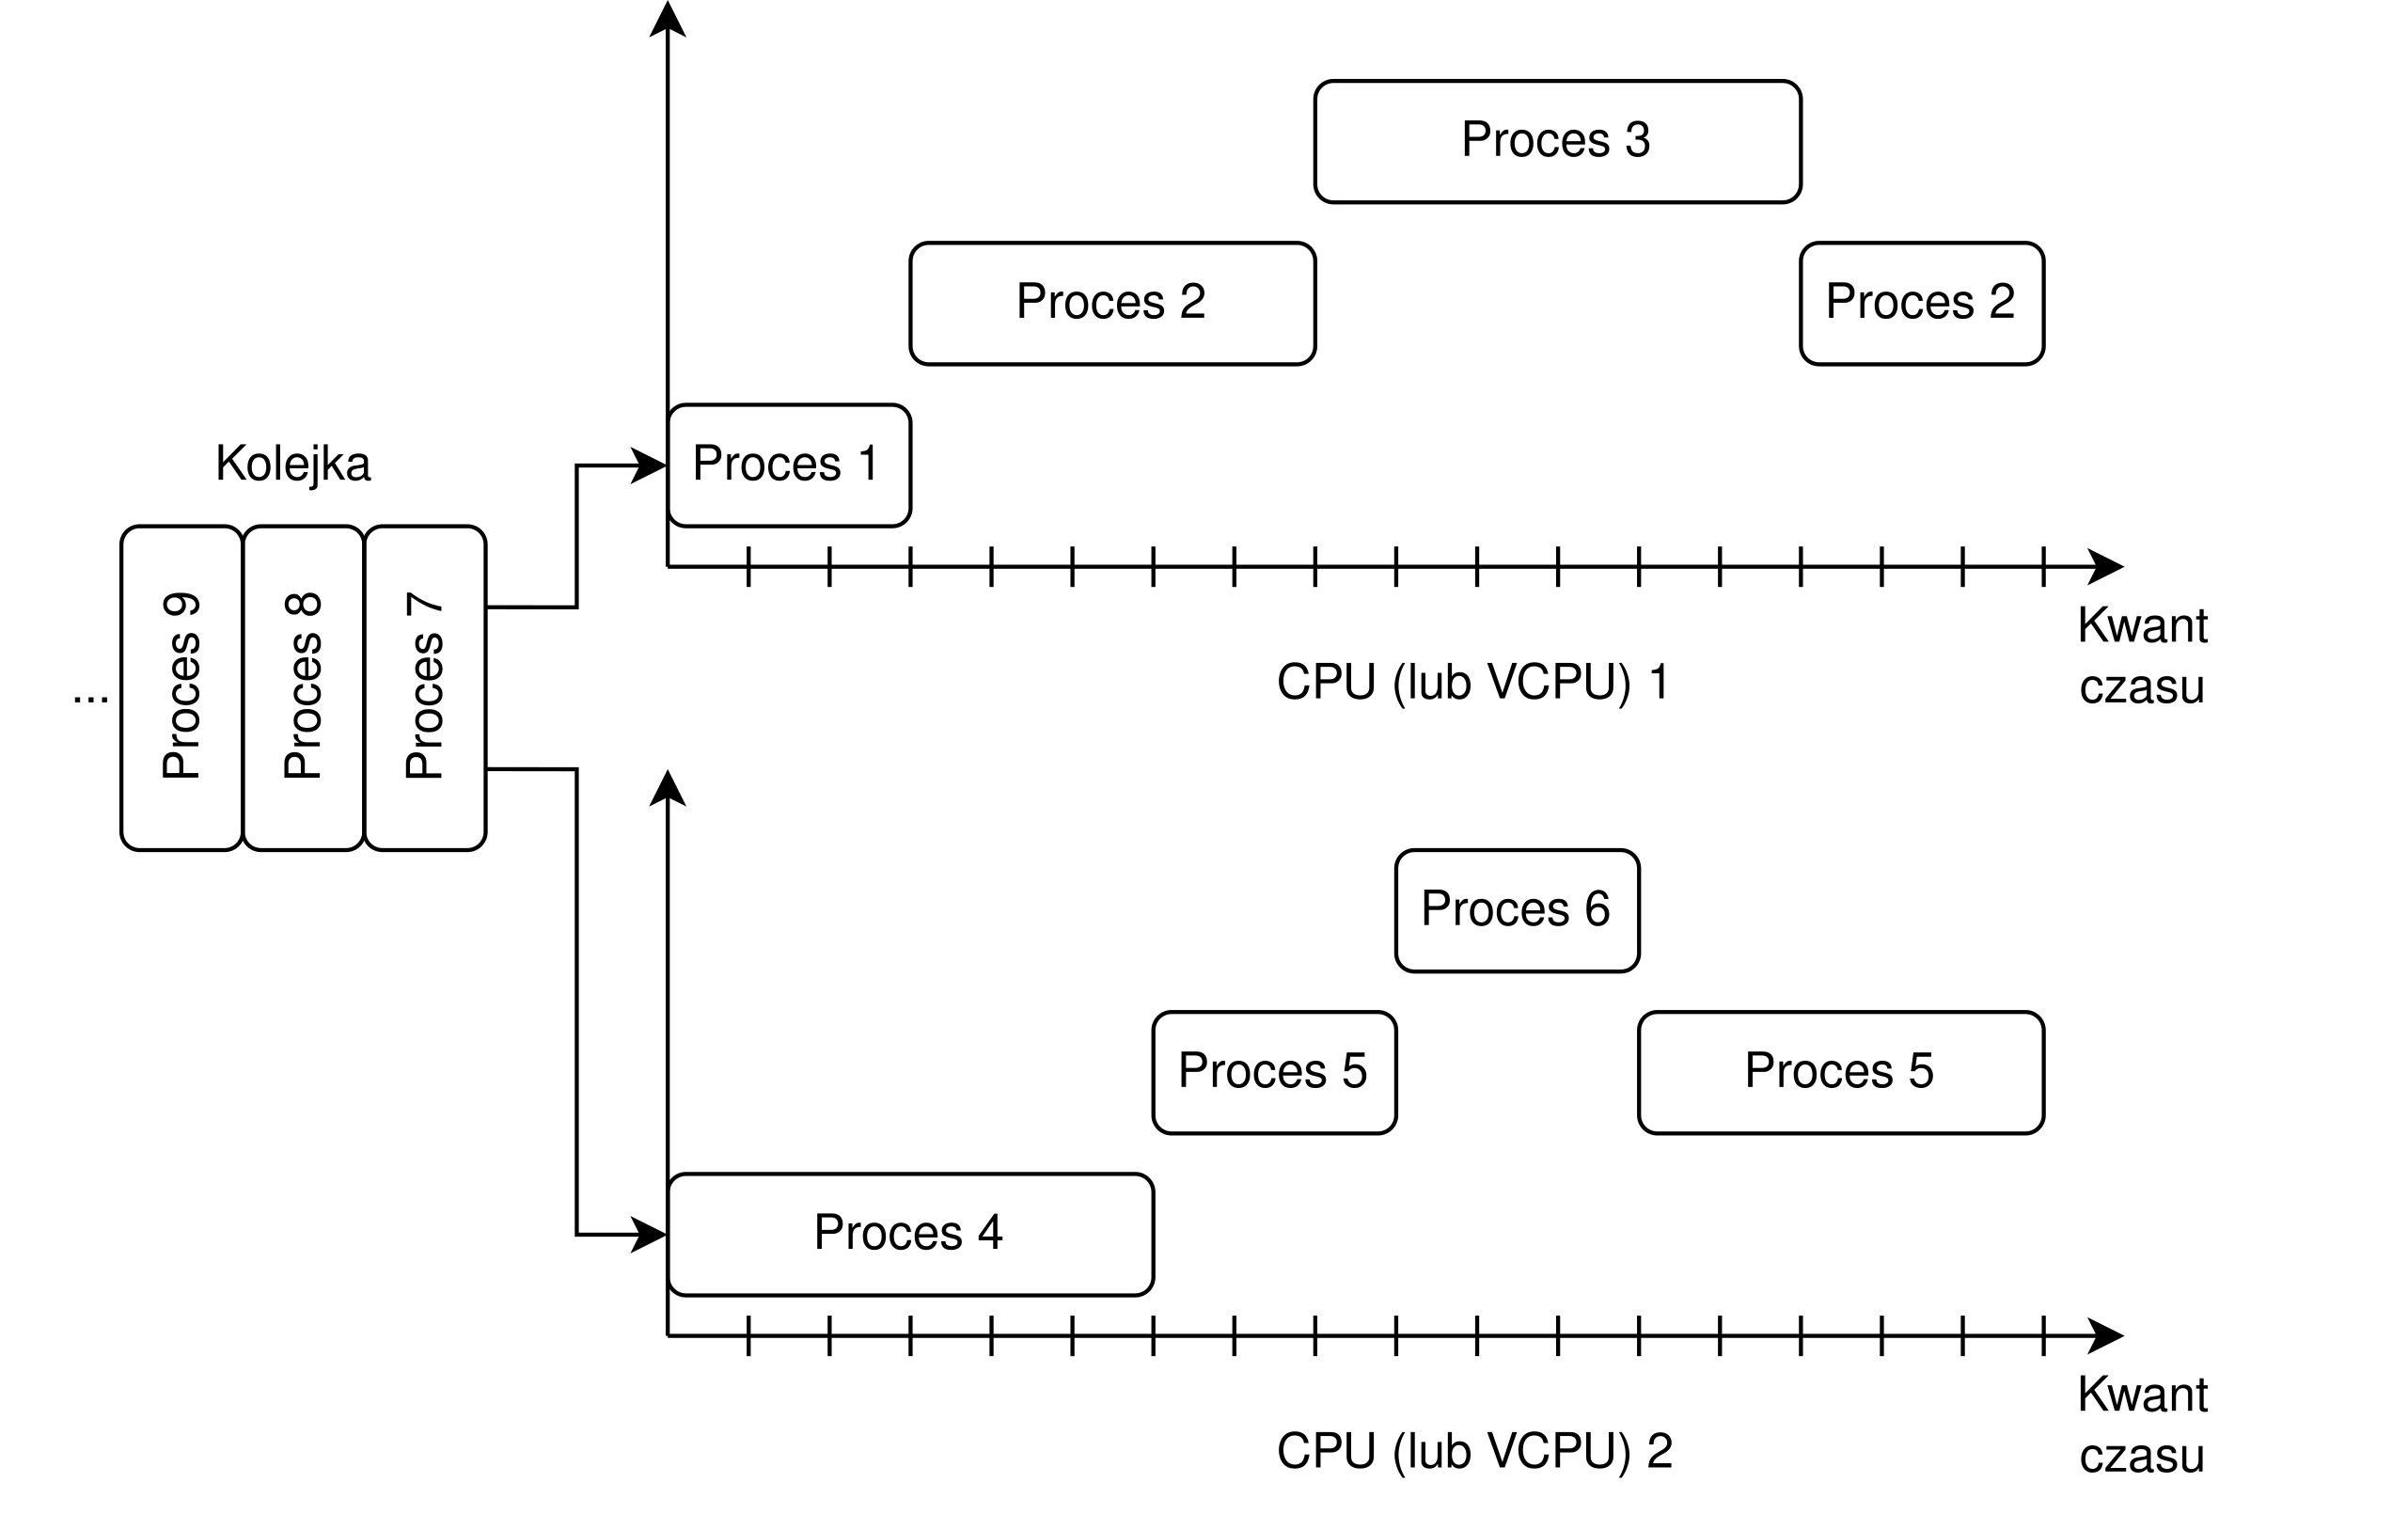
\includegraphics[width=0.95\textwidth]{Images/time-sharing.png}
    \caption{Współdzielenie zasobów jednostek obliczeniowych przez wiele procesów w technologii AMP}
    \label{fig:time-sharing}
\end{figure}

W przypadku, gdy jest kilka jednostek obliczeniowych dostępnych dla wszystkich programów, zarządzanie ich zasobami można zorganizować na dwa sposoby: przydzielać każdemu programowi czas oddzielnej jednostki obliczeniowej (techniki \gls{amp}) lub połączyć zasoby wszystkich jednostek obliczeniowych i przydzielać jednemu programowi pewną część  tych zasobów(techniki \gls{smp}).

W przypadku wirtualizacji programom udostępniane są \gls{vcpu}. Są to w pewnym sensie przerobione przez hiperwizor zasoby realnej jednostki obliczeniowej.

Na \cref{fig:time-sharing} przedstawiono przykład współdzielenia zasobów jednostek obliczeniowych przez wiele procesów w technologii \gls{amp}. Każdemu procesowi przypisana jest pewna część zasobów obliczeniowych, reprezentowana przez liczbę kwantów czasu (ang. time slice; najmniejsza możliwa ilość czasu jednostki obliczeniowej, którą można przypisać procesu w niektórych realizacja oprogramowania systemowego).

Stąd można zrobić trzy wnioski:

\begin{enumerate}
    \item Zasobem jednostki obliczeniowej jest jej czas;
    \item Czas może być przypisywany bezpośrednio lub podzielony przez oprogramowanie systemowe na pewne minimalne odcinki: kwanty czasu;
    \item W przypadku obecności wielu jednostek obliczeniowych, zarządzanie ich zasobami odbywa się zgodnie z technikami \gls{amp} lub \gls{smp}.
\end{enumerate}

\end{document}